\section{Capítulo 6: Confiabilidad y tolerancia a fallos}

\textbf{Confiabilidad:} La confianza que se puede tener en un sistema, aun en presencia de errores, fallos y condiciones inesperadas.

Atributos claves

\begin{enumerate}
    \item \textcolor{red}{\textbf{Fiabilidad:}} Continuidad correcta del servicio sin fallas o interrupciones.
    \item \textcolor{red}{\textbf{Disponibilidad:}} La disposición de un servicio a ser usado en cualquier tiempo \textbf{T} .
    \item \textcolor{red}{\textbf{Mantenibilidad:}} Facilidad de mantener, actualizar y reparar un sistema que puede fallar.
    \item \textcolor{red}{\textbf{Protección:}} Ausencia de consecuencias catastróficas sobre el medio ambiente.
    \item \textcolor{red}{\textbf{Seguridad}} Prevenir el acceso o manipulación no autorizaco (alineado con la \textcolor{red}{\textbf{CIA: Confidencialidad, Integridad y Disponibilidad}}).
\end{enumerate}

Los atributos antes mencionados son cuantificables y medibles para el analisis de la \textbf{tolerancia a fallos}.

\subsection{Modelo Causal de averias}
Para este contexto definiremos al sistema como un conjunto de componentes tanto de hardware como de software, preparados para colaborar coordinadamente para ofrecer un servicio, según pautas establecidas para un correcto funcionamiento.


Pero, que causa un mal funcionamiento de un sistema. Partiremos definiendo 3 diferencias claves para el analisis.

\begin{itemize}
    \item \textcolor{red}{\textbf{Fallo(\textit{fault}):}} Defecto o funcionamiento anormal de un componente, el cual tiene el potencial de causar un \textcolor{red}{\textbf{error}}, en caso de no ser tratado \textcolor{red}{\textbf{puede llevar a una averia}}. Se clasifican segun persistencia (\textcolor{red}{\textbf{transistente, intermitente o permanente}}) y según causa \textcolor{red}{\textbf{error de manofactura, diseño u operacional}} 
    \item \textcolor{red}{\textbf{Error:}} Discrepancia entre el comportamiento esperado y el exhibido
    \item \textcolor{red}{\textbf{Averia(\textit{failture}):}} Ocurre un malfuncionamiento que conduce a que ya no se pueda proveer el servicio especificado. Son causadas por errores que se propagar a lo largo del sistema, llegando a ser observables por el usuario.
    \subitem \textbf{Un error o fallo no necesariamente conduce a una averia, si este es tratado y manejado adecuadamente}
\end{itemize}

Las \textbf{\textit{fallas}} o \textbf{\textit{averias}} se clasifican según su comportamiento en el sistema

\begin{itemize}
    \item Fallas de \textcolor{red}{\textbf{caida (\textit{crash}):}} Componente se detiene y no se recupera por si mismo
    \subitem \textcolor{red}{\textbf{Proceso:}} Proceso fallado se detiene, puede perder su estado. Es la mas benigna es detenerse manteniendo su estado, para posteriormente recuperarlo. Para la detenccion fiable por parte de otros procesos se requieren \textcolor{red}{\textit{timers}}
    \subitem \textcolor{red}{\textbf{Comunicación:}} Falla del sistema de comunicación con pérdida continua de mensajes (e.g falla permanenete o partición de red)

    \item Fallas de \textcolor{red}{\textbf{omisión:}} El sistema no responde transitoriamente
    \subitem \textcolor{red}{\textbf{Proceso:}} Proceso no responde, sin perder estado \textcolor{red}{(e.g., se pierde una solicitud de servicio)}.
    \subitem \textcolor{red}{\textbf{Comunicación:}} Se pierden algunos mensajes. Falla mas benigna es que mensajes no se corrompen (integridad) y no se puede falsear su
    remitente (autenticidad). Recuperación es por retransmisión de mensajes perdidos.

    \item Fallas \textcolor{red}{\textbf{temporales (\textit{timing}):}} El sistema no responde dentro de los limites de tiempo.
    \subitem Pueden corresponder a un mal desempeño por sobrecarga. 
    \subitem Pueden ocurrir por fallas de relojes.

    \item Fallas \textcolor{red}{\textbf{arbitrarias (\textit{bizantinas}):}} El sistema se comporta inconsistente o maliciosamente.
    \subitem Los procesos fallas siguen funcionando pero no garantizan la integridad de los mensajes \textcolor{red}{\textbf{(peor caso)}}
    \subitem A veces se produce por corrupción interna del sistema, causan respuestas erroneas pero no maliciosas
    \subitem Son fallas dificiles de detectar y tolerar
\end{itemize}


Una vez definidas el tipo de fallas, estableceremos los modelos para los tipos de fallas, en base a una jerarquia.

\begin{itemize}
    \item \textcolor{red}{\textbf{Fail-stop:}} Un proceso fallado se detiene, conservando su estado, y todos los demas saben inmediatamente que ha fallado. Los procesos se comportan correctamente o se detienen.
    \item \textcolor{red}{\textbf{Crash:}} Modelo realista de incertidumbre para sistemas asincronicos. Un proceso fallad se detiene, conserva su estado, pero los demans no lo saben ni estan seguros si se cayo o esta lento o tiene problemas de comunicación. Puede recuperarse y reintegrarse al sistema
    \item \textcolor{red}{\textbf{Omisión:}} Solo un proceso puede omitir enviar o recibir mensajes. Se puede abordar con el uso de timers, reintento y asentimientos.
    \item \textcolor{red}{\textbf{Temporal (\textit{timing}):}} El sistema puede violar restricciones temporales, tal como respuestas fuera de tiempo. Dificil de discriminar entre fallas de crash y omisión
    \item \textcolor{red}{\textbf{Bizantino:}} Un proceso puede enviar mensajes contradictorios, mentir sobre su estado interno o colaborar maliciosamente con otros. Corresponde a un modelo más general
\end{itemize}

\begin{figure}[H]
    \centering
    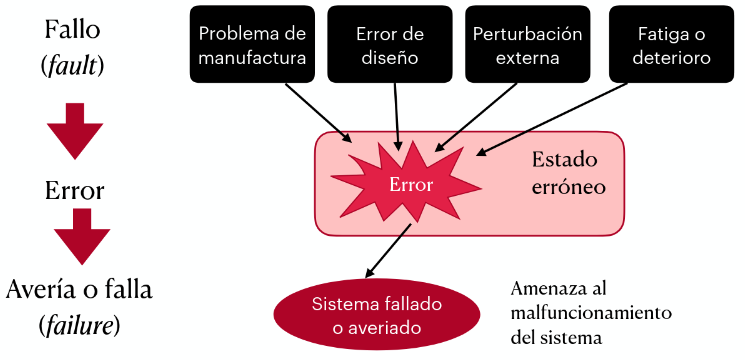
\includegraphics[width=0.48\linewidth]{img/Modelo_Causal_de_averias.png}
    \caption{Modelo Causal de averias}\label{fig:1761579857293}
\end{figure}


Para manejar lo anterior, se propone los siguientes enfoques para mejorar la confiabilidad del sistema.

\begin{itemize}
    \item \textcolor{red}{\textbf{Prevención de fallos:}} Prevenir que ocurran o se introduzcan fallos en el sistema
    \item \textcolor{red}{\textbf{Remoción de fallos}} durante el desarrollo o durante el uso \textbf{(mantencion y reparacion)}
    \item \textcolor{red}{\textbf{Pronóstico de fallos:}} Predecir fallos probables, para que puedan ser anticipadamente eliminadas o contener sus efectos \textbf{(e.g. alertas y detección de degradación/anomalías)}
    \item \textcolor{red}{\textbf{Pronóstico de fallos:}} Capacidad de un sistema para seguir funcionando normalmente, aun cuando seproduzcan uno o más fallos de sus componentes.
    \subitem Se debe disponer de algún tipo de redundancia para enmascarar fallos.
    \subitem Capacidad de reparar un fallo sin interrumpir el servicio, para asegurar continuidad operacional del servicio.
\end{itemize}

\subsection{Tolerancia a fallos}
Definimos la tolerancia a fallos como la capacidad de enmascarar la existencia de fallos en un sistema, usando redundacia. Esto busca evitar una averia o falla del sistema. Si bien un sistema puede ser tolerante a fallos, estos deberian ser de sus propios componentes, y no con fallas que comprometen todo el sistema. Queremos que el sistema, a pesar de que sus componentes esten fallados, este tenga un comportamiento consistente a lo especificado.
\vspace{1mm}

El manejo de fallos en un sistema es un proceso de cuatro fases: primero, la \textbf{Detección de error}, donde los fallos se deducen por errores en el estado del sistema; segundo, la \textbf{Aislación y evaluación del daño}, que busca contener la expansión del error; tercero, la \textbf{Recuperación del error}, que corrige el problema y devuelve el sistema a un estado consistente (e.g., \textit{rollback}); y finalmente, el \textbf{Tratamiento del fallo y servicio contínuo}, que, ante fallos permanentes, reconfigura el sistema para dejar de usar el componente dañado y reemplazarlo.

La \textcolor{red}{\textbf{redundancia}} se define en base a las partes de un sistema que no son necesarias para su correcto funcionamiento, si no se requiere tolerar fallos. Existen 3 tipos de tolerancias
\begin{enumerate}
    \item \textbf{Espacial:} Se agregan componentes de redundantes de hardware o software.
    \item \textbf{Temporal:} Ejecutar y repetir varias veces una acción o secuencia de instrucciones (similar a la maquina de estado determoinista y replicada). Un ejemplo es la retransmisión de mensajes, rollback de una acción y repetir su ejecición.
    \item \textbf{De información:} Se agrega información redundante para tolerar fallos.
\end{enumerate} 

\subsection{Enfoques de recuperación de errores}
Para recuperarnos de errores durante la ejecución tenemos dos enfoques.

\textbf{Recuperación regresiva(\textit{backward recovery}):} El sistema retrocede a un estado correcto anterior y se repite la ejecución, se introduce el concepto de checkpoints en la ejecución, los cuales son puntos donde se guarda el estado del sistema en una memoria estable (no se ve afectada por alguna averia). En caso de detectar errores, el sistema hace un rollback.

\textbf{Recuperación progresiva(\textit{forward recovery}):} El sistema sigue avanzando, corrigiendo un posible estado erroneo. Al detectarse errores, se siguie si ejecución mientras que a la par se realizan acciones correctivas. No es viable para todos los sistemas

\begin{figure}[H]
    \centering
    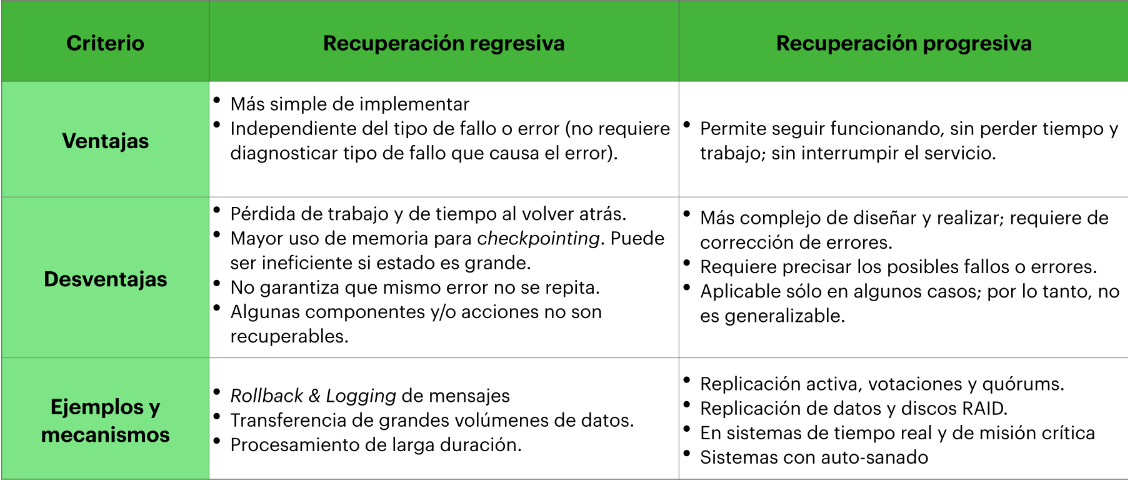
\includegraphics[width=1\linewidth]{img/Comparacion_enfoques.png}
    \caption{Comparativa de enfoques de recuperación}\label{fig:1761609494042}
\end{figure}

Dentro de los esquemas para tolerancia a fallos encontramos 
\begin{itemize}
    \item Transacciones o acciones atomicas
    \item Checkpoint y rollback
    \item Replicación de procesos
    \item Maquina de estado replicada o determoinista
    \subitem Basada en multicast atomico con orden total
    \subitem Ordenamiento basado en conceso (Paxos,Raft)
\end{itemize}

\subsection{Maquina de estado determinista y replicada}
Esta maquina es un grupo de replicación, donde cada proceso no fallado, ejecuta los mismos comandos en el mismo orden. Se caracteriza por el determinismo de estado, donde todas las replicas correctas mantienen el mismo estado. Se necesita concenso (dińamico) de los miembros del grupo, este consenso es sobre \textcolor{red}{\textbf{cúales comandos ejecutar y en que orden}}. Se trabaja sobre modelos con o sin fallas donde, si se trabaja en un modelo \textbf{sin fallas}, se pueden usar relojes de lampor para ordenamiento global y total de los mensajes del grupo o un secuenciador central. Para el caso del modelo con fallas, se requieren de algoritmos de consesso tolerantes a fallos. 

Para un ejemplo vamos a considerar lo siguiente, un contador $k$, el cual es iniciado con un valor de 1, tendremos dos maquinas que ejecutaran las mismas instrucciones, pero en diferente orden, para este caso:

\textcolor{red}{\textbf{Maquina A:}}
\begin{itemize}
    \item Multiplicar por 2 a $k$
    \item Sumarle 1 a $k$
\end{itemize}
\textcolor{red}{\textbf{Maquina B:}}
\begin{itemize}
    \item Sumarle 1 a $k$
    \item Multiplicar por 2 a $k$
\end{itemize}
\vspace{1mm}

Esto resulta en que al final el contador de la maquina A, sera \textcolor{red}{$k=3$} y para la maquina B, el \textcolor{red}{$k=4$}. por esto buscamos mantener un orden y los mismos comandos para ambas maquinas.

\subsection{Modelos cuantitativos de confiabilidad}
%Pagina 21
Se define la \textbf{fiabilidad R(t)} como la probabilidad de que un sistema no falle hasta el timepo t. Tambien definimos \textbf{MTTF (Mean Time To Failure)} como el tiempo de vida esperado sin un fallo del sistema. la cual se calcula de la siguiente forma:

\[
    MTTF= \int_{0}^{\infty}R(t)dt
\]

Para un caso especial, donde $R(t)$ sigue una distribución exponencial tenemos que $R(t)=\exp^{-\lambda t}$ y $MTTF= \frac{1}{\lambda}$

\subsubsection{Fiabilidad en serie}
Un sistema en serie, es aquel en donde si un componente falla, el sistema completo falla. Donde $R_i(t)$ es la fiabilidad del componente i, y $\lambda_i$ es la tasa media de fallas de componentes, de lo anterior la fiabilidad del sistema completo es:

\[
    R_{serie}=\prod_{i=1}^{n} R_i(t)
\]
Para un caso especial, donde $R(t)$ sigue una distribución exponencial tenemos que $R(t)=\exp^{-\lambda t}$ y $MTTF_{serie}= \frac{1}{\lambda}$ con $\lambda= \sum_{i=1}^{n}\lambda_i $ 

\subsubsection{Fiabilidad en paralelo}
Un sistema en paralelo, es aquel donde si \textbf{TODOS} los componentes del sistema, el sistema falla (Se mantendra la misma notación que anteriormente definida)

\[
    R_{paralelo}= 1 - \prod_{i=1}^{n} (1-R_i(t))
\]

Para un caso especial, donde $R(t)$ sigue una distribución exponencial tenemos que $R(t)=\exp^{-\lambda t}$ y $MTTF_{serie}= \frac{1}{\lambda}*\frac{ln(n)}{\lambda}$ con $\lambda= \sum_{i=1}^{n}\lambda_i $

\subsubsection{Confiabilidad con cadenas de Markov}
Modelo de fallas que tolera una única falla y con una reparación, se plantea la siguiente solución, considerando que $MTTF=\frac{1}{\lambda}$ y que $MTTR=\frac{1}{\mu}$
\begin{figure}[H]
    \centering
    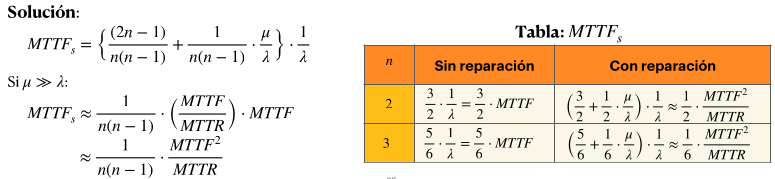
\includegraphics[width=1.0\linewidth]{img/Markov.png}
    \caption{Solución y dos ejemplos}\label{fig:1761834118505}
\end{figure}

\subsubsection{Caso de fiabilidad en discos raid-4 y espejo}

\begin{figure}[H]
    \centering
    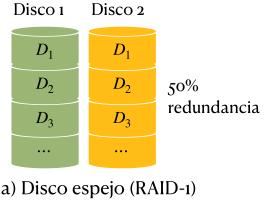
\includegraphics[width=1.0\linewidth]{img/Espejo.png}
    \caption{Ejemplo disco espejo}\label{fig:1761834250462}
\end{figure}
Para este caso el $MTTF\approx\frac{1}{2}*\frac{MTTF^2}{MTTR}$


\begin{figure}[H]
    \centering
    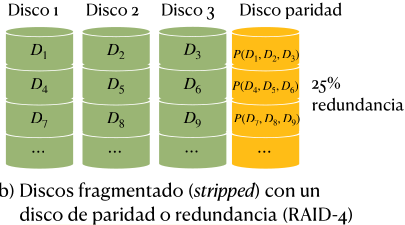
\includegraphics[width=1.0\linewidth]{img/Raid-4.png}
    \caption{Ejemplo para discos fragmentados RAID-4}\label{fig:1761834325234}
\end{figure}

Para este caso el $MTTF\approx\frac{1}{n(n-1)}*\frac{MTTF^2}{MTTR}$. El funcionamiento de este ultimo considera que se almacenan grupos de K bloques de datos y el uno de módulo dos (XOR) para el calculo de paridad. De lo anterior, se define lo siguiente para el calculo del bloque de datos $D_i$

\[
    D_i = D_1 \oplus D_2 \oplus \dots \oplus D_{i-1} \oplus D_{i+1} \oplus \dots \oplus D_k \oplus P
\]

\subsection{Disponibilidad}
Se definira la disponibilidad instantanea como $A(T)$ como la probabilidad de que un sistema este funcionamiento correctamente en un tiempo T. Luego la disponibilidad limite, se define como un valor $\alpha$, como la disponibilidad promedio en un invervalo $[0,\tau)$ como:
\[
    \alpha= \lim_{\tau \rightarrow \infty} \frac{1}{\tau}\int_{0}^{\tau}A(t)dt
\]

Aca se comienza a hablar sobre el concepto de reparacion, de la cual definimos el siguiente "flujo" (Notar que ahora un componente tiene 2 estados, reparandose y funcionando). de la cual se extrae lo siguiente:
\begin{figure}[H]
    \centering
    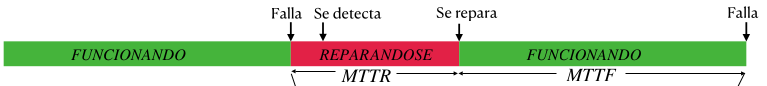
\includegraphics[width=1.0\linewidth]{img/MTTF.png}
    \caption{Flujo de vida de un componente}\label{fig:1761836148913}
\end{figure}
de lo anterior definimos que MTTF corresponde al "Mean Time TO Failure", MTBF como "Mean Time Between Failure" y MTTR como "Mean Time To Repair", donde tenemos finalmente que $MTBF= MTTF + MTTR$. Adicionalmente, podemos encontrar la disponibilidad limite $\alpha$ como:

\[
    \alpha = \frac{MTTF}{MTTF+MTTR}
\]

\subsubsection{Caso de replicación de servidores}
Suponiendo un sistema de n réplicas similares, donde la disponibilidad por servidor es de $a_0$ , donde se trabaja con un modelo en paralelo, la solucion de disponibilidad es $a_n=1-(1-a_0)^n$

\subsection{Acuerdo y consenso distribuido}
Para el consenso  en sistemas distribudios es fundamental mantener consistencia y confiabilidad en el sistema, es decir mantener un estado consistente y funcionar correctamente en presencia de fallas, particiones de red y/o retardos. El objetivo de los algoritmos asociados al tema es garantizar el acuerdo entre nodos sobre un unico valor o tomar una misma decisión. Los desafios principales son la falla en nodos, particiones de red, comunicación asincrona (Demora en mensaje, cambio de orden o perdida de los mismos), y las fallas bizantinas.

En el problema del acuerdo, se busca decidir sobre un único valor o curso de acción tal que se satisfaca el \textbf{acuerdo} (el valor decidido debe ser igual para todos), \textbf{integridad} (no se puede cambiar la decisión de un participante), \textbf{valides}(el valor elegido debio ser propuesto por alguno de los participales) y\textbf{termino} (se decide en tiempo finito). Todo esto sobre el ambiente de fallas anteriormente planteado. Notar que las tres primeras condiciones hacen referencia a \textbf{\textit{safety}} y la última a \textbf{\textit{liveness}}
\textbf{Acuerdo.} Existe un proceso designado (transmisor) que tiene y propone un valor inicial, para alcanzar acuerdo con los demás procesos sobre este valor, según las siguientes condiciones:
\begin{itemize}
    \item \textbf{Acuerdo:} Todos los procesos no fallados tienen que acordar el mismo valor.
    \item \textbf{Validez:} Si el proceso transmisor está no fallado, entonces el valor acordado por todos los procesos no fallados tiene que ser el mismo valor inicial del transmisor.
\end{itemize}

\textbf{Consenso.} Cada proceso tiene un valor inicial y todos los procesos correctos tienen que acordar un único valor, según las siguientes condiciones:
\begin{itemize}
    \item \textbf{Acuerdo:} Todos los procesos no fallados tienen que acordar el mismo valor (único).
    \item \textbf{Validez:} Si todos los procesos no fallados tienen el mismo valor inicial, entonces el valor acordado tiene que ser este valor; o alguno de los valores iniciales, si los valores no son iguales.
\end{itemize}

\textbf{Consistencia interactiva.} Cada proceso tiene un valor inicial y todos los procesos correctos tienen que acordar sobre un conjunto de valores, según las siguientes condiciones:
\begin{itemize}
    \item \textbf{Acuerdo:} Todos los procesos no fallados tienen que acordar el mismo arreglo de valores $A[v_1, v_2, \dots, v_n]$.
    \item \textbf{Validez:} Si proceso $P_i$ no fallado tiene valor inicial $v_i$, entonces todos los procesos no fallados acordará $v_i$ como el valor $A[i]$ (\textit{nótese}: si proceso $P_j$ está fallado, entonces todos los procesos no fallados acordarán cualquier valor común para $A[j]$).
\end{itemize}

Para la relación entre procesos se sigue la siguiente relacion de componentes en buen estado y fallados $f<n$ (varia segun el modelo de fallas). Para la existencia de solucion debe de existir comunicación fiable, en caso de que es sistema sea asincrónico, no es posible llegar a una solucion, dado que no se puede discriminar entre falla o demora.

\subsubsection{Algoritmo de acuerdo bizantino con mensajes ordinarios (no tienen ningún hash criptografico)}

Para este algoritmo, solo se trabaja con un modelo de fallas bizantinas y no de comunicación, donde se debe cumplir que $3f+1\leq n$ . Para el numero m de rondas, se cumple que existe a lo mas $m= f+1$ rondas.

Para la primera ronda (el caso base $m = 0$), el transmisor envía su valor a todos los receptores (nodos), seguido a eso, cada receptor usa el valor recibido del transmisor o el por defecto.

Para las siguientes rondas (los pasos recursivos $m > 0$), el transmisor envía el valor a los receptores, \textbf{y cada receptor ($P_i$) anota ese valor ($v_i$)} (o usa el valor por defecto si no recibe nada). Inmediatamente, ese mismo receptor $P_i$ actúa como un nuevo transmisor en una \textbf{sub-ronda} del algoritmo (específicamente $OM(f-1)$), y le envía \textit{su} valor $v_i$ a todos los demás $n-2$ receptores.

Finalmente, después de esa sub-ronda, cada receptor $P_i$ recopila todos los valores ($v_j$) que recibió de sus compañeros. El valor que $P_i$ decide y adopta como final es el que gane por \textbf{mayoría} entre todos los valores que juntó ($v_1, \dots, v_{n-1}$). (se explica mejor visualizando el algoritmo la verdad)

\begin{figure}[H]
    \centering
    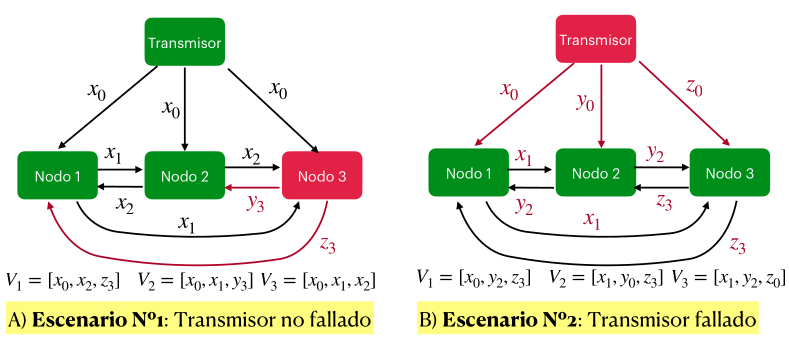
\includegraphics[width=1.0\linewidth]{img/ordinario.png}
    \caption{Ejemplo de OM con n=4 y f=1}\label{fig:1761838884075}
\end{figure}

\subsection{Comunicación grupal tolerante a fallos}
El principal enfoque es que claro, una vez tengamos el mecanismo necesitamos las herramientas (replicación de maquina de estado, \textit{primary-backup}, sistemas basados en quorums) para la replicación de los datos.

Estan presentes dos tipos de multicast.
\textbf{Simple:}  No esta determinado el número de receptores efectivos, cuando existen emisores de uno o varios, no esta determinado el orden de llegada a los receptores, es util para apliicaciones no críticas, no tiene condiciones de consistencia, es mas eficiente o liviano

\textbf{Fiable:} Garantiza la entrega a procesos no fallados aun en presencia de de fallos de comunicación. Se retransmiten mensajes automáticamente, elimiando mensajes repetidos o corruptos.

\begin{figure}[H]
    \centering
    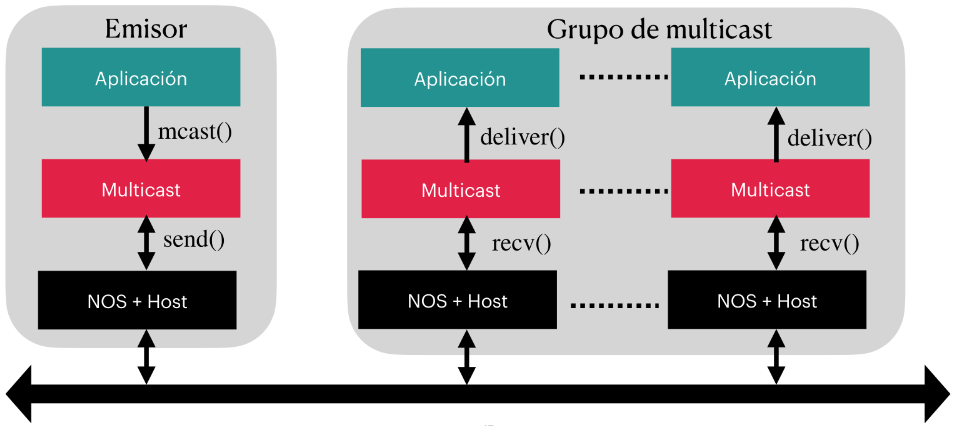
\includegraphics[width=1.0\linewidth]{img/Multicast_grupal.png}
    \caption{Usando comunicación grupal (multicast)}\label{fig:1761651184845}
\end{figure}
\subsubsection{Semantica de dentrega de mensajes}
\textbf{Fiabilidad de entrega:}
\begin{itemize}
    \item \textbf{Mejor esfuerzo} (Best-effort): Sin garantía sobre cuántos miembros reciben un mensaje.
    \item \textbf{Fiabilidad-}$k$: Garantía de que al menos $k$ miembros reciben el mensaje.
    \item \textbf{Atómico}: Garantía de que todos los miembros lo reciben, o ninguno de ellos lo recibe.
\end{itemize}
\textbf{Orden de entrega:}
\begin{itemize}
    \item \textbf{No ordenado}: Ninguna garantía de orden de entrega en el receptor.
    \item \textbf{Orden FIFO}: Mensajes de un mismo emisor se entregan según orden de envío.
    \item \textbf{Orden causal}: Se respeta en la entrega orden causal de eventos de envío.
    \item \textbf{Orden total}: Único orden de entrega de los mensajes en los receptores. Podría requerir también cumplir orden causal.
\end{itemize}

\begin{figure}[H]
    \centering
    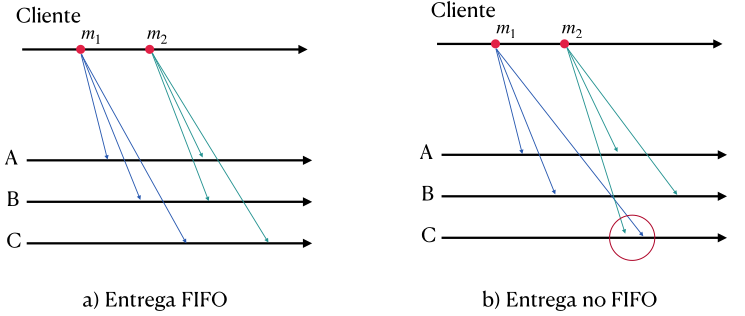
\includegraphics[width=0.7\linewidth]{img/multi_fifo.png}
    \caption{Multicast: orden FIFO}\label{fig:1761678535409}
\end{figure}

\begin{figure}[H]
    \centering
    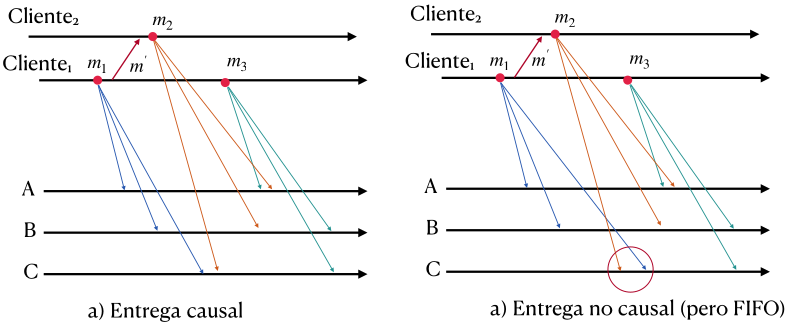
\includegraphics[width=0.7\linewidth]{img/multi_causal.png}
    \caption{Multicast: orden causal}\label{fig:1761678585653}
\end{figure}

\begin{figure}[H]
    \centering
    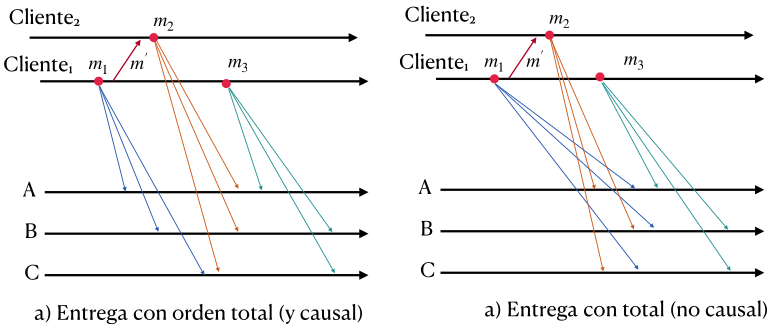
\includegraphics[width=0.7\linewidth]{img/multi_total.png}
    \caption{Multicast: orden total}\label{fig:1761678629682}
\end{figure}

\textcolor{red}{\textbf{Obs.1:}} Es necesario utlizar multicas con entrega con orden total y causal pasa maquinas de estado replicadas deterministas para asegurar la entrega de comandos en el mismo orden.

En los grupos muchas veces existen miembros distinguidos (con un rol asociado), los nodos, deben tomar el rol del nodo afectado una vez detectada la falla. Si en algún punto un nuevo nodo se integra al grupo, se debe sincronizar con los demás nodos
\subsubsection{Modelo de sincronia virtual (modelo \textit{Fail-stop})}
Definimos la sincronia virtual como un modelo de comunicación que asegura consistencia de entrega de mensajes aun en presencia de fallos. Es facil de implementar una maquina de estado replicada y determinista y replicada  en un modelo \textit{Fail-stop} multicast fiable y cambios de mebresía. Algo a tener en cuenta es que este modelo no soporta fallas bizantinas ni particiones de red.

El sistema es parcialmente asincronico porque requiere de \textit{timer} para detectar la falla de procesos 

\textbf{ABCAST:} Asegura orden total, tiene la semantica de entrega más fuerte. Para que un grupo reciba un mensaje en el mismo orden, se necesita un protocolo de dos fases, para este caso el proceso que manda un mensaje actúa como "coordinador", va a actuar en el grupo para determinar el orden en que deben de llegar los mensajes desde este coordinador, utiliza relojes de lamport y el id del proceso, como un par ordenado de la forma $\left[LC, \textit{pid}\right]$, se maneja una cola para garantizar la condición de entrega ordenada.

En su primera fase $P_i$ va a enviar un mensaje usando multicast fiable, una vez enviado el mensaje, el resto de los procesos del grupo (no fallados), marca tentativamente los mensajes recibidos en base a su reloj local de lamport $\left[LC_j, id_j\right]$, finalmente para cada mensaje recibido por el proceso $P_i$, los asigna como \textbf{No comprometido}, \textcolor{red}{(en la imagen, los mensajes con la N)}. En la segunda fase, una vez $P_i$ reciba la marca tentativa de sus miembros del grupo, marca la máxima marca tentativa como $t_m$, (en caso de que dos procesos tengan el mismo valor para el relojes, se desempata con el id). Finalmente una vez definido el valor para el mensaje, Se le notifica a todos los procesos del grupo, la marca ganadora y se pasa el valor de comprometido a \textcolor{blue}{\textbf{TRUE}}.

\textbf{Primera fase}
\begin{figure}[H]
    \centering
    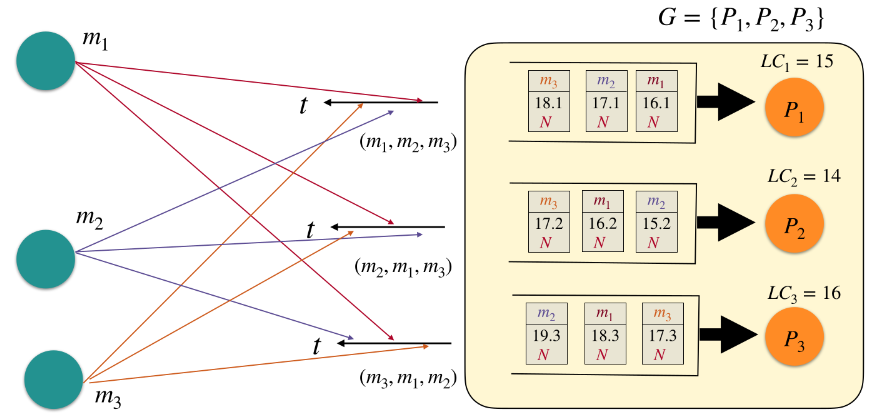
\includegraphics[width=0.7\linewidth]{img/Primer_paso.png}
    \caption{Primer paso ABCAST}\label{fig:1761653095435}
\end{figure}

\begin{figure}[H]
    \centering
    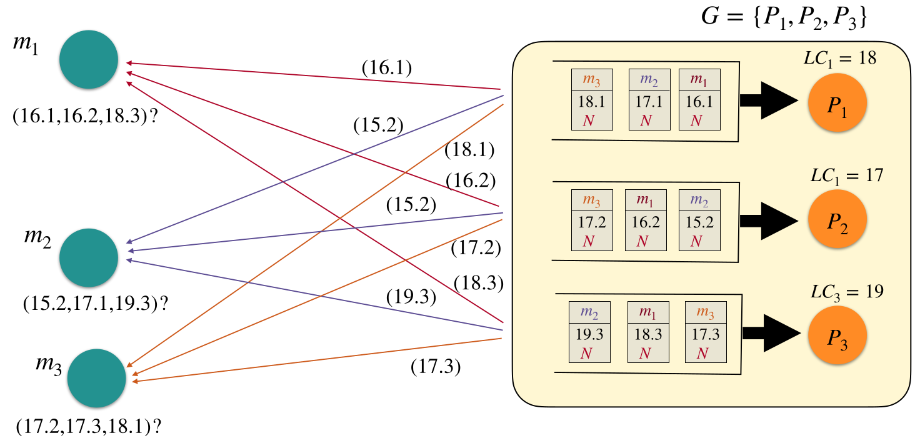
\includegraphics[width=0.7\linewidth]{img/Segundo_paso.png}
    \caption{Segundo paso ABCAST}\label{fig:1761653127112}
\end{figure}

\textbf{Segunda fase}

\begin{figure}[H]
    \centering
    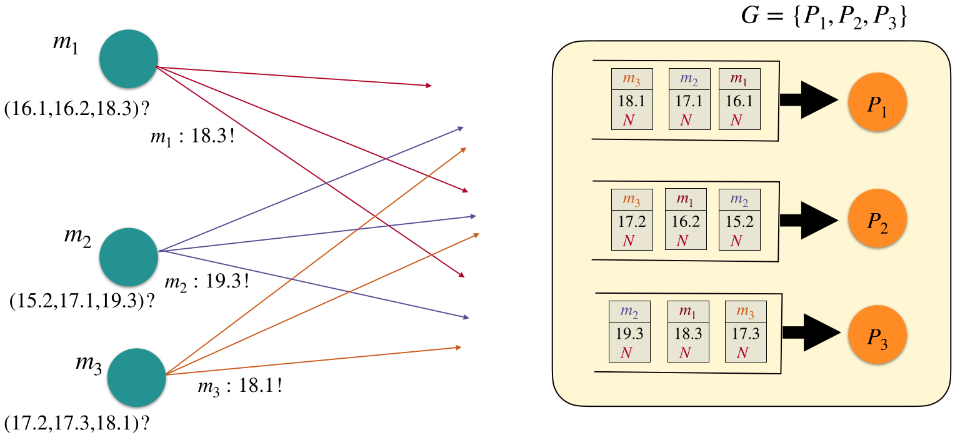
\includegraphics[width=0.7\linewidth]{img/Tercer_paso.png}
    \caption{Tercer paso ABCAST}\label{fig:1761653161267}
\end{figure}

\begin{figure}[H]
    \centering
    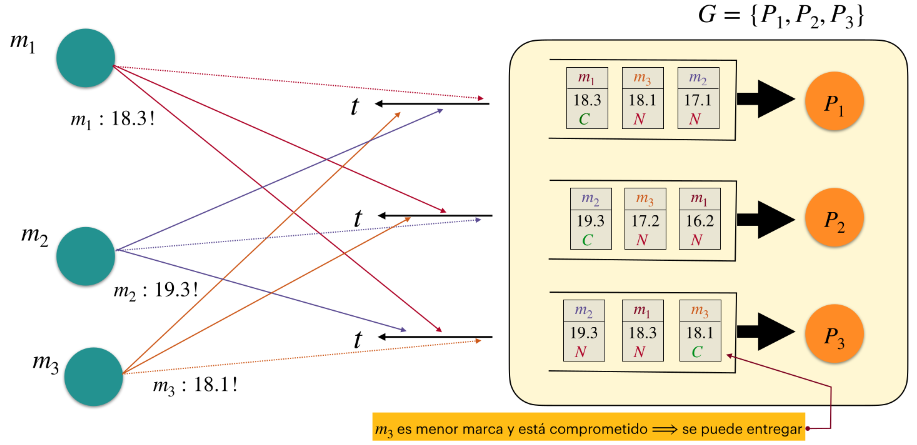
\includegraphics[width=0.7\linewidth]{img/Cuarto_paso.png}
    \caption{Cuarto paso ABCAST}\label{fig:1761653182730}
\end{figure}

Para establecer un numero de mensajes por solicitud, Si hay N procesos, hay N envios, Como hay N procesos, hay N respuestas, y finalmente Se tiene que comunicar para los N procesos N actualizaciones de marca para un mensaje, resultando finalmente en que la \textcolor{red}{complejidad} es $3N$


\textbf{CBCAST:} Asegura orden causal, hace uso de relojes vectoriales,antes habia un solo monitor, y cada miembro hace entrega causal. Las reglas son las siguientes. Para cada mensaje m, a ser enviado por $P_i$, se incrementa $VC_i[i]$, Cuando $P_j$,  recibe un mensaje m desde $P_i$, con la marca asociada al mensaje, entonces $P_j$ retarda la entrega de m hasta que se cumpla la condicion \textcolor{red}{\textbf{FIFO}} y la condicion \textcolor{red}{\textbf{CAUSAL}} (estas se definieron en el capitulo 4, y están en este apunte).

\begin{figure}[H]
    \centering
    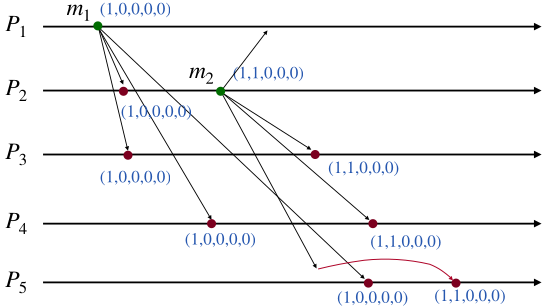
\includegraphics[width=0.7\linewidth]{img/CBCAST.png}
    \caption{Ejemplo visual de CBCAST}\label{fig:1761675486364}
\end{figure}

\textbf{Api de gestion de grupos:} Pasa asegurar atomicidad, nos provee una interfaz para gestionar grupos, servicios como, crear grupo, unirse a un grupo, salir de un grupo (por detección termino o fallas), una lista de quienes reciben el mensaje (Vista), y notificar un cambio de en la lista del grupo.

Definimos un grupo atomico, como un grupo donde todos los miembros tienen la misma vista, cuando existen cambios en la vista (alguien se sale o une al grupo), este proceso necesariamente debe ser atómico.

\begin{figure}[H]
    \centering
    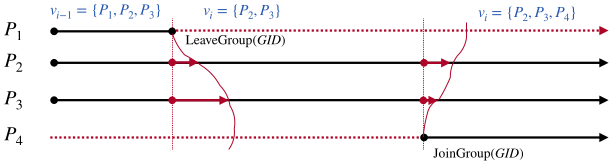
\includegraphics[width=1.0\linewidth]{img/Api_gestion.png}
    \caption{Ejemplo de grupos atomicos para API de gestión de grupos}\label{fig:1761676301300}
\end{figure}

\textcolor{red}{\textbf{Obs.1}} Notar que los 3 protocolos antes descritos tienen entrega atómica.


\subsection{Algoritmo de PAXOS y otros (consenso con fallas de crash)}

Paxos se usa para mantener consistente información del sistema, por ejemplo, información de la configuración del sistema. Permite coordinacion tolerante a fallos.

